\documentclass[11pt,a4paper]{article}

% ── Packages ───────────────────────────────────────────────
\usepackage[T1]{fontenc}
\usepackage{newtxtext,newtxmath}
\usepackage[a4paper,margin=2.5cm,headheight=14pt]{geometry}
\usepackage{microtype}
\usepackage{amsmath}
\usepackage{booktabs,tabularx,longtable}
\usepackage[group-separator={,},group-minimum-digits=4]{siunitx}
\usepackage{graphicx}
\usepackage[font=small,labelfont=bf,skip=6pt]{caption}
\usepackage{xcolor}
\usepackage{enumitem}
\usepackage{titlesec}
\usepackage{fancyhdr}
\usepackage[authoryear,round]{natbib}
\usepackage[colorlinks=true,linkcolor=accent,citecolor=accent,urlcolor=accent]{hyperref}

\definecolor{accent}{HTML}{1F3A5F}
\definecolor{muted}{HTML}{5B6470}

\titleformat{\section}{\large\bfseries\color{accent}}{\thesection}{0.8em}{}
\titleformat{\subsection}{\normalsize\bfseries}{\thesubsection}{0.8em}{}
\titlespacing*{\section}{0pt}{1.6em}{0.6em}
\titlespacing*{\subsection}{0pt}{1.1em}{0.4em}

\setlist{itemsep=2pt,topsep=4pt}
\setlength{\parskip}{4pt}
\setlength{\parindent}{0pt}

\pagestyle{fancy}
\fancyhf{}
\fancyhead[L]{\small\color{muted}Vessel Age Curve (M1) -- Technical Note}
\fancyhead[R]{\small\color{muted}Yan Li}
\fancyfoot[C]{\small\color{muted}\thepage}
\renewcommand{\headrulewidth}{0.4pt}

\newcommand{\usd}[1]{\text{US\$}#1}
\newcommand{\age}{\mathrm{age}}

% ── Document ───────────────────────────────────────────────
\begin{document}

\begin{titlepage}
\vspace*{3cm}
{\color{accent}\rule{\linewidth}{1pt}}\\[0.8em]
{\LARGE\bfseries Vessel Age Curve (M1)}\\[0.4em]
{\Large Valuing a second-hand ship from comparable sales}\\[0.6em]
{\color{accent}\rule{\linewidth}{1pt}}\\[1.5em]
{\large Technical note: model specification, estimation, application and back-test}\\[3em]

\begin{tabular}{@{}ll@{}}
Author & Yan Li \\
Case & Target Ship 1, MR product tanker, built 2012 \\
Valuation date & 22 May 2026 \\
Version & 1.1 (12 November 2026) \\
\end{tabular}

\vfill
\begin{minipage}{\linewidth}
\small
\textbf{Summary.}
The model values a second-hand ship from recent sales of similar ships. Sale prices are first moved to the valuation date with a broker price benchmark; an exponential depreciation curve is then fitted to price against age by ordinary least squares on log price, and the ship is read off the curve at its own age.
Only sales reported on or before the valuation date are used. On 43 MR tanker sales the curve explains 91\% of the variation in log price and implies that value falls by 8.4\% for each additional year of age.
Target Ship 1, aged 14, is valued at \usd{29.67}m (range \usd{26.27}--33.06m); its reported sale price of \usd{28.45}m lies 4.1\% below the fitted value and inside the range.
A leave-one-out back-test gives an average absolute error of 7.5\% and a bias of $+0.8\%$.

\textit{Version 1.1 removes hindsight: version 1.0 used 30 sales, four of them reported after the valuation date (value \usd{29.52}m). Earlier broker reports were added instead.}
\end{minipage}
\end{titlepage}

\tableofcontents
\newpage

% ───────────────────────────────────────────────────────────
\section{Purpose and scope}

The model answers one question: \emph{what is a given ship worth on a given date, judged by what similar ships have recently sold for?}
It is the first model in a ship valuation portfolio and supplies the market value used by the later models (discounted cash flow valuation, acquisition and financing, build versus buy).

\begin{table}[h]
\centering
\caption{Inputs and outputs.}
\label{tab:io}
\begin{tabularx}{\linewidth}{@{}XX@{}}
\toprule
Inputs & Outputs \\
\midrule
Recent sales of the same ship type: age, price, sale date & Market value (\usd{}m) \\
A broker price benchmark, to move prices to one date & Range around the value \\
Age of the ship on the valuation date & Value lost per year of age \\
 & Goodness of fit ($R^2$) \\
 & Test against a known price, where one exists \\
\bottomrule
\end{tabularx}
\end{table}

\textbf{Scope.} The method is applied here to MR product tankers (about 45,000--55,000 dwt). Age is the only explanatory variable; size, yard, survey timing and fuel efficiency are treated in a separate hedonic regression model (M1+).

% ───────────────────────────────────────────────────────────
\section{Method and terminology}

The model combines three standard elements:

\begin{description}[leftmargin=0pt,font=\normalfont\bfseries]
\item[Comparable sales method (market approach).] The asset is valued by reference to prices paid for similar assets, adjusted for differences in date and characteristics \citep{IVS105}.
\item[Exponential (geometric) depreciation.] Value is assumed to fall by a constant \emph{percentage} per year of age. Constant-rate depreciation is the pattern found in the classic studies of second-hand asset prices \citep{HultenWykoff1981a,HultenWykoff1981b}.
\item[Log-linear regression by ordinary least squares.] Taking logarithms turns the exponential curve into a straight line, which is estimated by ordinary least squares (OLS).
\end{description}

The model is the one-variable case of a \emph{hedonic} price regression, in which the price of a good is explained by its characteristics \citep{Court1939,Griliches1961,Rosen1974}. Applied to ships, the same framework has been used to value vessels from cross-sectional sales data \citep{AdlandKoekebakker2007}.

% ───────────────────────────────────────────────────────────
\section{Data}

\subsection{Selection of comparables}

Sales are collected from weekly broker sale-and-purchase reports and screened with written rules:
\begin{itemize}
\item same ship type and size band (MR product tanker);
\item an exact reported price (indicative prices such as ``low \usd{20}s'' are excluded);
\item no sale with an attached charter, no resale of a newbuilding contract, no repeated entry;
\item the sale was reported on or before the valuation date (no information from after that date is used);
\item the ship being valued is excluded from its own comparables.
\end{itemize}
For Target Ship 1 this leaves $n = 43$ sales reported between December 2025 and May 2026, aged 5 to 20 years at sale. The data are listed in Appendix~\ref{app:data}.

\subsection{Adjustment to the valuation date}

Each reported price is moved to the valuation date $T$ with a broker benchmark for a ship of similar age:
\begin{equation}
\label{eq:index}
P_i = P_i^{\text{rep}} \times \frac{B(T,\,k_i)}{B(t_i,\,k_i)},
\end{equation}
where $P_i^{\text{rep}}$ is the reported price of sale $i$, $t_i$ its date, and $B(t,k)$ the benchmark price on date $t$ for benchmark age $k \in \{5, 10, 15\}$ years, choosing the benchmark age nearest the ship's age at sale.

\emph{Example.} Sale~03, a 14-year-old ship, was reported at \usd{27.60}m. The 15-year benchmark rose by 11.8\% between its sale date and 22 May 2026, giving an adjusted price of \usd{30.85}m.
In what follows, ``price'' means the adjusted price $P_i$.

% ───────────────────────────────────────────────────────────
\section{Model specification}

\subsection{Exponential depreciation curve}

If a ship loses a constant fraction of its value for each year of age, value follows
\begin{equation}
\label{eq:curve}
P = a\,e^{\,b\,\age},
\end{equation}
where $a > 0$ is the level of the curve at age zero and $b < 0$ its rate of decline.
The curve falls steeply at young ages and flattens later, because a constant percentage loss is a smaller dollar amount on a cheaper ship.

\subsection{Log-linear form}

Taking natural logarithms of \eqref{eq:curve}, using $\ln(xy) = \ln x + \ln y$ and $\ln e^{z} = z$, gives
\[
\ln P = \ln a + \ln e^{\,b\,\age} = \ln a + b\,\age .
\]
Writing $c = \ln a$ and adding an error term $\varepsilon_i$ for everything age does not explain, the estimating equation for sale $i$ is
\begin{equation}
\label{eq:model}
\boxed{\;\ln P_i = c + b\,\age_i + \varepsilon_i, \qquad i = 1,\dots,n.\;}
\end{equation}
This is a straight line with dependent variable $\ln P$ and explanatory variable age, and it is the equation the model estimates.

% ───────────────────────────────────────────────────────────
\section{Estimation}

\subsection{Ordinary least squares}

OLS chooses $c$ and $b$ to minimise the sum of squared errors
\begin{equation}
\label{eq:sse}
S(c,b) = \sum_{i=1}^{n} \bigl(\ln P_i - c - b\,\age_i\bigr)^2 .
\end{equation}
At the minimum both partial derivatives are zero. By the chain rule, the derivative of a squared term is twice the term times the derivative of its inside, so
\begin{align}
\frac{\partial S}{\partial c} &= -2\sum_{i} \bigl(\ln P_i - c - b\,\age_i\bigr) = 0, \label{eq:foc_c}\\
\frac{\partial S}{\partial b} &= -2\sum_{i} \age_i\bigl(\ln P_i - c - b\,\age_i\bigr) = 0. \label{eq:foc_b}
\end{align}
Dividing \eqref{eq:foc_c} by $-2n$ gives the intercept,
\begin{equation}
\label{eq:c}
\hat c = \overline{\ln P} - \hat b\,\overline{\age},
\end{equation}
so the fitted line passes through the point of means. Substituting \eqref{eq:c} into \eqref{eq:foc_b} and rearranging gives the slope,
\begin{equation}
\label{eq:b}
\hat b = \frac{\sum_i (\age_i - \overline{\age})(\ln P_i - \overline{\ln P})}{\sum_i (\age_i - \overline{\age})^2}
= \frac{S_{xy}}{S_{xx}},
\end{equation}
the sample covariance of age and log price divided by the sample variance of age.

\subsection{Returning to price}

Exponentiating the fitted line, using $e^{\ln x} = x$ and $e^{m+n} = e^m e^n$,
\[
\hat P = e^{\hat c + \hat b\,\age} = e^{\hat c}\, e^{\hat b\,\age} = \hat a\, e^{\hat b\,\age}, \qquad \hat a = e^{\hat c}.
\]
By the power-of-a-power rule $(x^m)^n = x^{mn}$, read in reverse, $e^{\hat b\,\age} = (e^{\hat b})^{\age}$. Defining the annual factor $\hat r = e^{\hat b}$,
\begin{equation}
\label{eq:rform}
\boxed{\;\hat P = \hat a\,\hat r^{\,\age}.\;}
\end{equation}

\subsection{Interpretation of the parameters}

\begin{table}[h]
\centering
\caption{Parameters and their meaning.}
\label{tab:params}
\begin{tabularx}{\linewidth}{@{}l l X@{}}
\toprule
Symbol & Definition & Meaning \\
\midrule
$b$ & slope of $\ln P$ on age & change in log price per additional year of age \\
$r = e^{b}$ & annual factor & share of value retained by a ship one year older \\
$1 - r$ & annual depreciation & percentage of value lost per additional year \\
$-b$ & approximation to $1-r$ & from $e^{b} = 1 + b + b^2/2 + \cdots \approx 1 + b$ for small $b$ \\
$a = e^{c}$ & level at age zero & scale constant of the curve; not a newbuilding price (Section~\ref{sec:interp}) \\
\bottomrule
\end{tabularx}
\end{table}

\subsection{Fit, value and range}

Goodness of fit is measured on the log scale:
\begin{equation}
\label{eq:r2}
R^2 = 1 - \frac{\sum_i (\ln P_i - \widehat{\ln P_i})^2}{\sum_i (\ln P_i - \overline{\ln P})^2}.
\end{equation}
The market value of a ship of age $\age_0$ is $V = \hat a\,\hat r^{\,\age_0}$. The reported range is $V \pm \mathrm{SD}$, where SD is the sample standard deviation of the dollar residuals $P_i - \hat P_i$.

% ───────────────────────────────────────────────────────────
\section{Application: Target Ship 1}

\textbf{Case.} Target Ship 1 is an MR product tanker built in 2012 at a South Korean yard, of about 52,000 dwt, aged 14 years on the valuation date of 22 May 2026. Its sale was reported at \usd{28.45}m. Because the ship is excluded from its own comparables, this price provides an independent test of the model.

\subsection{Estimates}

\begin{table}[h]
\centering
\caption{Estimation on 43 MR sales.}
\label{tab:est}
\begin{tabular}{@{}l l r@{}}
\toprule
Quantity & Calculation & Value \\
\midrule
Number of comparables & & 43 \\
Mean age & $\overline{\age}$ & 15.163 \\
Mean log price & $\overline{\ln P}$ & 3.28800 \\
Cross-product sum & $S_{xy}$ & $-50.1705$ \\
Sum of squared age deviations & $S_{xx}$ & 571.860 \\
\midrule
Slope & $\hat b = S_{xy}/S_{xx}$ & $\mathbf{-0.08773}$ \\
\quad standard error & & 0.00429 \\
\quad 95\% confidence interval & & $[-0.0964,\ -0.0791]$ \\
Intercept & $\hat c = \overline{\ln P} - \hat b\,\overline{\age}$ & \textbf{4.61826} \\
Level at age zero & $\hat a = e^{\hat c}$ & 101.32 \\
Annual factor & $\hat r = e^{\hat b}$ & 0.9160 \\
Annual depreciation & $1 - \hat r$ & \textbf{8.4\%} \\
\quad 95\% confidence interval & & 7.6\%--9.2\% \\
Goodness of fit & $R^2 = 1 - 0.43056/4.83213$ & \textbf{0.911} \\
\bottomrule
\end{tabular}
\end{table}

The fitted curve is
\[
\hat P = 101.32 \times 0.9160^{\,\age}.
\]
The slope is estimated precisely ($t = -20.5$): with 95\% confidence, value falls by between 7.6\% and 9.2\% per year of age.

\subsection{Valuation}

\[
\ln V = 4.61826 - 0.08773 \times 14 = 3.39001, \qquad V = e^{3.39001} = \usd{29.67}\text{m},
\]
equivalently $101.32 \times 0.9160^{14} = \usd{29.67}$m.

\begin{table}[h]
\centering
\caption{Valuation of Target Ship 1 on 22 May 2026.}
\label{tab:value}
\begin{tabular}{@{}l r@{}}
\toprule
Output & Value \\
\midrule
Market value & \textbf{\usd{29.67}m} \\
Standard deviation of residuals & \usd{3.40}m \\
Range ($\pm$ 1 SD) & \usd{26.27}m -- \usd{33.06}m \\
Cross-check: mean of the 7 sales within $\pm$1 year of age 14 & \usd{30.32}m \\
\midrule
Reported sale price & \usd{28.45}m \\
Reported minus fitted & $-\usd{1.22}$m ($-4.1\%$) \\
Reported price inside the range & Yes \\
\bottomrule
\end{tabular}
\end{table}

\begin{figure}[h]
\centering
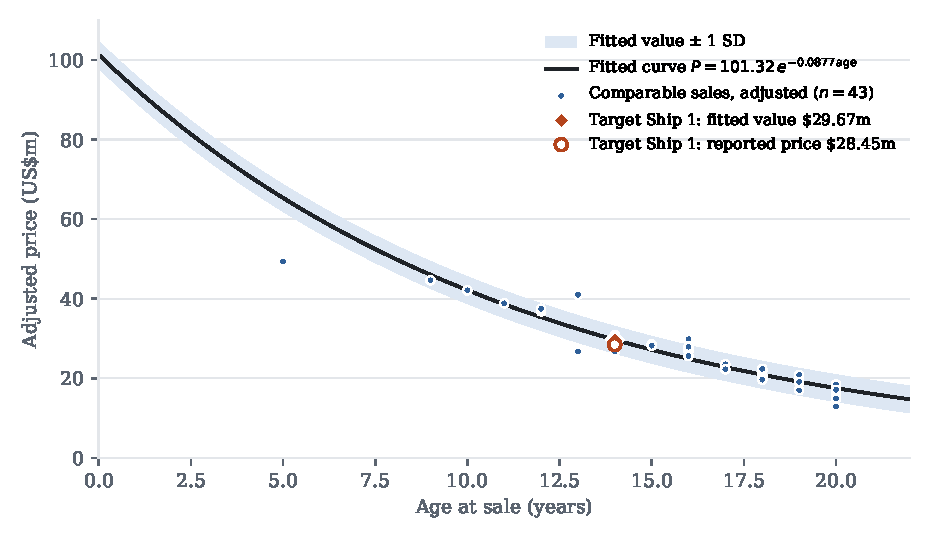
\includegraphics[width=\linewidth]{figures/age_curve.pdf}
\caption{Fitted age curve on 43 MR sales adjusted to 22 May 2026, with the $\pm$1 SD range and Target Ship 1.}
\label{fig:curve}
\end{figure}

% ───────────────────────────────────────────────────────────
\section{Interpretation}
\label{sec:interp}

\begin{itemize}
\item \textbf{Value.} On recent MR sales, a 14-year-old MR tanker was worth about \usd{29.7}m on 22 May 2026.
\item \textbf{The reported price was close to market.} At \usd{28.45}m it is 4.1\% below the curve and well inside the range: neither a distressed sale nor an overpayment.
\item \textbf{Depreciation of about 8\% per year.} A 15-year-old MR is worth $0.916$ times a 14-year-old, about \usd{27.2}m. Because the loss is proportional, the dollar loss shrinks with age: \usd{2.72}m from age 13 to 14 and \usd{2.49}m from 14 to 15.
\item \textbf{Age explains 91\% of the variation in log price.} The remaining 9\% reflects yard, size, condition, survey timing, fuel efficiency and deal terms, which this model does not measure.
\item \textbf{Cross-check.} The seven sales closest in age average \usd{30.32}m, within 2.2\% of the curve.
\end{itemize}

\textbf{The level at age zero is not a newbuilding price.} $\hat a = \usd{101.32}$m, whereas a new MR tanker cost about \usd{50}m in May 2026 according to broker newbuilding benchmarks. The youngest comparable is five years old, so the curve below that age extrapolates the 9--20-year trend. $\hat a$ should be read only as the scale constant of \eqref{eq:rform}.

\textbf{The annual factor is cross-sectional.} $\hat r$ compares ships of different ages at the same date. It is not a forecast of one ship's price a year later, which also depends on how the market moves.

% ───────────────────────────────────────────────────────────
\section{Back-test}

\subsection{Design}

A back-test applies the model to prices that are already known, as if they were unknown, and compares its answers with the actual prices.
In a \emph{leave-one-out} back-test each sale is valued by a curve estimated without it, so that no sale contributes to its own valuation. This mirrors how the model is used: valuing a ship that is not in the data. For each $i = 1, \dots, n$:
\begin{enumerate}
\item remove sale $i$;
\item estimate $\hat c_{(-i)}$ and $\hat b_{(-i)}$ by \eqref{eq:c}--\eqref{eq:b} on the remaining $n-1$ sales;
\item value sale $i$: $\hat P_{(-i)} = \exp\bigl(\hat c_{(-i)} + \hat b_{(-i)}\,\age_i\bigr)$;
\item record the error $e_i = \hat P_{(-i)}/P_i - 1$ (positive when the model is too high).
\end{enumerate}

\emph{Example.} Without Sale~01 (17 years, \usd{23.50}m) the curve is $101.40 \times 0.9159^{\age}$, which gives \usd{22.78}m at age 17: an error of $-3.1\%$.

\subsection{Error measures}

The $n$ errors are summarised in two ways:
\begin{align}
\text{Average absolute error} &= \frac{1}{n}\sum_{i=1}^{n} \lvert e_i \rvert && \text{(accuracy of a single valuation)} \label{eq:mae}\\
\text{Bias} &= \frac{1}{n}\sum_{i=1}^{n} e_i && \text{(systematic over- or under-valuation)} \label{eq:bias}
\end{align}
The average absolute error is the primary measure, since a valuation concerns one ship. Bias alone can be zero while every valuation is wrong (errors of $+30\%$ and $-30\%$ average to zero); its role is to detect a one-sided tendency that could be corrected.

\subsection{Results}

\begin{table}[h]
\centering
\caption{Leave-one-out back-test on 43 MR sales.}
\label{tab:bt}
\begin{tabular}{@{}l r@{}}
\toprule
Measure & Result \\
\midrule
Average absolute error & \textbf{7.5\%} \\
Bias & $+0.8\%$ \\
Largest error & $+42.3\%$ (Sale 12, age 5) \\
Average absolute error excluding Sale 12 & 6.6\% \\
\bottomrule
\end{tabular}
\end{table}

\begin{figure}[h]
\centering
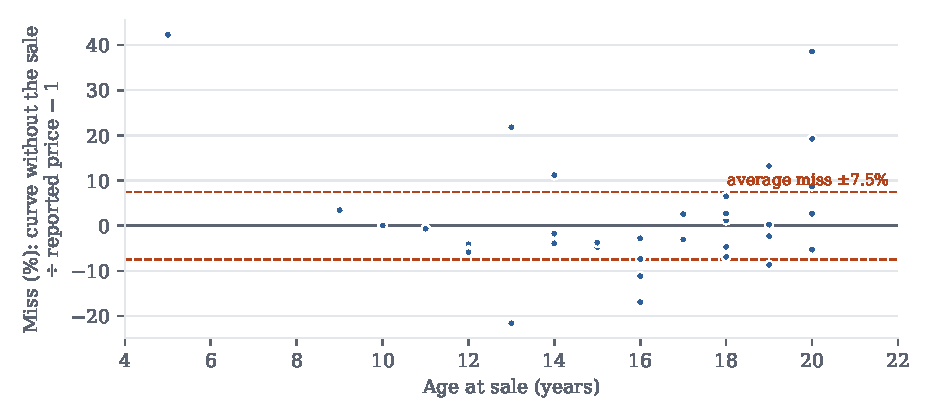
\includegraphics[width=\linewidth]{figures/backtest.pdf}
\caption{Leave-one-out errors by age. Dashed lines mark $\pm$ the average absolute error.}
\label{fig:bt}
\end{figure}

\begin{itemize}
\item \textbf{Accuracy.} A single valuation is typically within about 7.5\% of the actual price; for Target Ship 1 that is roughly $\pm$\usd{2.2}m.
\item \textbf{No systematic lean.} A bias of $+0.8\%$ indicates that the curve is neither consistently high nor low.
\item \textbf{The young end is weak.} The only sale under nine years (Sale 12, age 5) is overvalued by 42.3\%: without it, the curve extrapolated to age 5 gives \usd{70}m against an actual \usd{49}m. Valuations are reliable in the dense 9--20-year range and not below it.
\item \textbf{Single sales can miss widely.} The next largest errors are Sale 39 (age 20, $+38.6\%$), Sales 38 and 30 (age 13, $+21.8\%$ and $-21.6\%$) and Sale 24 (age 20, $+19.2\%$), where condition, survey timing and deal terms matter more than age alone. Sales from December and January also carry large time adjustments (up to $+39\%$), so any benchmark error passes into them.
\end{itemize}
Errors for every sale are listed in Appendix~\ref{app:data}.

% ───────────────────────────────────────────────────────────
\section{Limitations}

\begin{table}[h]
\centering
\caption{Limitations and remedies.}
\label{tab:limits}
\small
\begin{tabularx}{\linewidth}{@{}>{\raggedright\arraybackslash}X >{\raggedright\arraybackslash}X >{\raggedright\arraybackslash}X@{}}
\toprule
Limitation & Effect & Remedy \\
\midrule
Age is the only variable & Yard, size, survey timing, scrubber and fuel efficiency remain in the error & Hedonic regression (M1+) \\
No sales under five years & Young end of the curve and $\hat a$ are extrapolated & Newbuilding anchor; more young sales \\
One constant rate of depreciation & Actual values fall slowly at first and faster later & Non-linear or piecewise age term \\
En bloc sales entered separately & One deal at one price counts three times (Sales 04--06) or twice (Sales 18--19, 27--28, 40--41) & Treat an en bloc deal as one observation \\
Strong market rise December 2025 to May 2026 & Early sales are adjusted by up to $+39\%$; benchmark errors pass into them & Second-broker benchmark; shorter window as a test \\
Value read as $e^{\widehat{\ln P}}$ & Estimates the median; the mean is higher by about $e^{\hat\sigma^2/2} - 1 = 0.5\%$ & Smearing correction \citep{Duan1983} \\
Range is $\pm$1 SD of dollar residuals & Simple spread, not a formal interval; the 68\% prediction interval on log price is \usd{26.78}--32.87m & Prediction interval on log price \\
43 sales over five months & Estimates will move as data are added & Extend the sales register \\
\bottomrule
\end{tabularx}
\end{table}

% ───────────────────────────────────────────────────────────
\section{Conclusion}

A one-variable exponential depreciation curve, fitted by OLS on log price to 43 date-adjusted MR sales reported up to the valuation date, explains 91\% of the variation in log price and values Target Ship 1 at \usd{29.67}m, 4.1\% above its reported sale price and with the reported price inside the range. A leave-one-out back-test shows an average error of 7.5\% with negligible bias, and identifies the young end of the age range as the main weakness. The model provides a transparent, reproducible market value and a baseline for the hedonic regression (M1+), which adds the ship characteristics that age alone cannot capture.

% ───────────────────────────────────────────────────────────
\begin{thebibliography}{99}
\bibitem[Adland and Koekebakker(2007)]{AdlandKoekebakker2007}
Adland, R. and Koekebakker, S. (2007). Ship valuation using cross-sectional sales data: a multivariate non-parametric approach. \emph{Maritime Economics \& Logistics}, 9(2), 105--118.

\bibitem[Court(1939)]{Court1939}
Court, A. T. (1939). Hedonic price indexes with automotive examples. In \emph{The Dynamics of Automobile Demand}, 99--117. New York: General Motors Corporation.

\bibitem[Duan(1983)]{Duan1983}
Duan, N. (1983). Smearing estimate: a nonparametric retransformation method. \emph{Journal of the American Statistical Association}, 78(383), 605--610.

\bibitem[Griliches(1961)]{Griliches1961}
Griliches, Z. (1961). Hedonic price indexes for automobiles: an econometric analysis of quality change. In \emph{The Price Statistics of the Federal Government}, 173--196. New York: NBER.

\bibitem[Hulten and Wykoff(1981a)]{HultenWykoff1981a}
Hulten, C. R. and Wykoff, F. C. (1981a). The estimation of economic depreciation using vintage asset prices: an application of the Box--Cox power transformation. \emph{Journal of Econometrics}, 15(3), 367--396.

\bibitem[Hulten and Wykoff(1981b)]{HultenWykoff1981b}
Hulten, C. R. and Wykoff, F. C. (1981b). The measurement of economic depreciation. In C. R. Hulten (ed.), \emph{Depreciation, Inflation, and the Taxation of Income from Capital}, 81--125. Washington, DC: Urban Institute Press.

\bibitem[IVSC(2024)]{IVS105}
International Valuation Standards Council (2024). \emph{International Valuation Standards}, IVS 105: Valuation Approaches and Methods. London: IVSC.

\bibitem[Rosen(1974)]{Rosen1974}
Rosen, S. (1974). Hedonic prices and implicit markets: product differentiation in pure competition. \emph{Journal of Political Economy}, 82(1), 34--55.

\bibitem[Stopford(2009)]{Stopford2009}
Stopford, M. (2009). \emph{Maritime Economics}, 3rd ed. London: Routledge.

\bibitem[Tsolakis et al.(2003)]{Tsolakis2003}
Tsolakis, S. D., Cridland, C. and Haralambides, H. E. (2003). Econometric modelling of second-hand ship prices. \emph{Maritime Economics \& Logistics}, 5(4), 347--377.
\end{thebibliography}

\nocite{Stopford2009,Tsolakis2003}

% ───────────────────────────────────────────────────────────
\appendix
\section{Comparable sales and back-test errors}
\label{app:data}

Prices are adjusted to 22 May 2026 by \eqref{eq:index}. ``Curve without it'' is the leave-one-out valuation $\hat P_{(-i)}$.

\begin{center}
\small
\begin{longtable}{@{}l r r r r@{}}
\toprule
Sale & Age & Adjusted price (\usd{}m) & Curve without it (\usd{}m) & Error \\
\midrule
\endhead
Sale 01 & 17 & 23.50 & 22.78 & $-3.1\%$ \\
Sale 02 & 19 & 17.00 & 19.25 & $+13.2\%$ \\
Sale 03 & 14 & 30.85 & 29.64 & $-3.9\%$ \\
Sale 04 & 12 & 36.82 & 35.30 & $-4.1\%$ \\
Sale 05 & 12 & 36.82 & 35.30 & $-4.1\%$ \\
Sale 06 & 12 & 36.82 & 35.30 & $-4.1\%$ \\
Sale 07 & 19 & 19.00 & 19.14 & $+0.7\%$ \\
Sale 08 & 15 & 28.50 & 27.14 & $-4.8\%$ \\
Sale 09 & 20 & 16.21 & 17.62 & $+8.7\%$ \\
Sale 10 & 15 & 28.21 & 27.15 & $-3.8\%$ \\
Sale 11 & 16 & 26.82 & 24.85 & $-7.4\%$ \\
Sale 12 & 5 & 49.34 & 70.21 & $+42.3\%$ \\
Sale 13 & 9 & 44.61 & 46.14 & $+3.4\%$ \\
Sale 14 & 18 & 20.65 & 20.90 & $+1.2\%$ \\
Sale 15 & 18 & 20.36 & 20.91 & $+2.7\%$ \\
Sale 16 & 18 & 19.66 & 20.94 & $+6.5\%$ \\
Sale 17 & 16 & 25.59 & 24.87 & $-2.8\%$ \\
Sale 18 & 11 & 38.84 & 38.58 & $-0.6\%$ \\
Sale 19 & 11 & 38.84 & 38.58 & $-0.6\%$ \\
Sale 20 & 19 & 19.56 & 19.11 & $-2.3\%$ \\
Sale 21 & 14 & 30.18 & 29.65 & $-1.7\%$ \\
Sale 22 & 20 & 18.44 & 17.46 & $-5.3\%$ \\
Sale 23 & 16 & 27.94 & 24.82 & $-11.2\%$ \\
Sale 24 & 20 & 14.86 & 17.72 & $+19.2\%$ \\
Sale 25 & 12 & 37.34 & 35.27 & $-5.5\%$ \\
Sale 26 & 10 & 42.08 & 42.14 & $+0.2\%$ \\
Sale 27 & 17 & 22.24 & 22.82 & $+2.6\%$ \\
Sale 28 & 17 & 22.24 & 22.82 & $+2.6\%$ \\
Sale 29 & 10 & 42.12 & 42.14 & $+0.0\%$ \\
Sale 30 & 13 & 41.01 & 32.14 & $-21.6\%$ \\
Sale 31 & 19 & 20.85 & 19.05 & $-8.7\%$ \\
Sale 32 & 20 & 17.10 & 17.55 & $+2.7\%$ \\
Sale 33 & 12 & 37.48 & 35.27 & $-5.9\%$ \\
Sale 34 & 19 & 19.09 & 19.13 & $+0.2\%$ \\
Sale 35 & 16 & 29.83 & 24.78 & $-16.9\%$ \\
Sale 36 & 18 & 21.87 & 20.85 & $-4.7\%$ \\
Sale 37 & 14 & 26.76 & 29.75 & $+11.2\%$ \\
Sale 38 & 13 & 26.76 & 32.59 & $+21.8\%$ \\
Sale 39 & 20 & 12.91 & 17.90 & $+38.6\%$ \\
Sale 40 & 11 & 38.84 & 38.58 & $-0.6\%$ \\
Sale 41 & 11 & 38.84 & 38.58 & $-0.6\%$ \\
Sale 42 & 18 & 22.38 & 20.83 & $-6.9\%$ \\
Sale 43 & 16 & 27.94 & 24.82 & $-11.2\%$ \\
\midrule
\multicolumn{4}{@{}l}{Average absolute error / bias} & 7.5\% / $+0.8\%$ \\
\bottomrule
\end{longtable}
\end{center}

\section{Reproducibility}

All figures and numbers in this note are produced from \texttt{data/sample/comparables.csv} by \texttt{examples/run\_age\_curve.py} (model, back-test and charts in \texttt{src/vessel\_valuation/}), and agree to the cent with the Excel implementation of the model.
\end{document}
